\chapter{电动汽车群充电功率建模}
本文采用2009年全美家用车调查报告中的相关数据来描述电动汽车的出行特点。

\section{模型1}

\section{模型2}
利用数值算法求解时域积分方程,首先需要选取适当的空间基函数与时间基函数对待求感应电流进行离散。

\subsection{概率密度函数}
它的具体定义如下:
\begin{equation}
f_n(\bm{r})=
\begin{cases}
\frac{l_n}{2A_n^+}\bm{\rho}_n^+=\frac{l_n}{2A_n^+}(\bm{r}-\bm{r}_+)&\bm{r}\in T_n^+\\
\frac{l_n}{2A_n^-}\bm{\rho}_n^-=\frac{l_n}{2A_n^-}(\bm{r}_--\bm{r})&\bm{r}\in T_n^-\\
0&\text{otherwise}
\end{cases}
\end{equation}

其中,$l_n$为三角形单元$T_n^+$和$T_n^-$公共边的长度,$A_n^+$和$A_n^-$分别为三角形单元$T_n^+$和$T_n^-$的面积(如图\ref{pica}所示)。

\begin{figure}[h]
	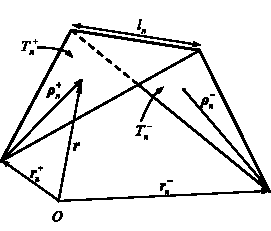
\includegraphics{pica.pdf}
	\caption{几何参数示意图}
	\label{pica}
\end{figure}

公式统一用英文斜体书写,公式中有上标、下标、顶标、底标等时,必须层次清楚。公式应居中放置,公式前的“解”、“假设”等文字顶格写,公式末不加标点,公式的序号写在公式右侧的行末顶边线,并加圆括号。序号按章排,如“(1-1)”、“(2-1)”。公式换行书写时与等号对齐。

公式2:
\begin{equation}
\label{latent_binary_variable}
\bm{r}_{i,j}=
\begin{cases}
1,f(\bm{x}^{i};\bm{w})\cdot f(\bm{x}^{j};\bm{w})\geq u(\lambda),\\
0,f(\bm{x}^{i};\bm{w})\cdot f(\bm{x}^{j};\bm{w})< l(\lambda), 1\leq i,j\leq n.\\
f(\bm{x}^{i};\bm{w})\cdot f(\bm{x}^{j};\bm{w}),\text{otherwise},
\end{cases}
\end{equation}

引用公式时应使用$\backslash$eqref 函数,用法和$\backslash$ref函数相同。

\subsection{其他基函数}

\subsubsection{特别提醒1}

\subsubsection{特别提醒2}

\section{考虑配电网不确定性的区间优化模型}

如图\ref{picb}和图\ref{picc}所示分别给出了参数$E_0=\hat{x}$,$a_n=-\hat{z}$,$f_0=\SI{250}{MHz}$,$f_w=\SI{50}{MHz}$,$t_w=4.2\sigma$时,配电网中的光伏、电动汽车和负荷都具有一定程度的不确定性。为保证优化模型的鲁棒性,本文以区间数来描述配电网中的不确定量,并采用区间潮流进行计算。区间数的计算法可参见文献,区间潮流的具体算法参见文献。第时刻光伏发电系统有功出力区间。

\begin{figure}[h]
	\begin{subfigure}[b]{0.49\linewidth}
		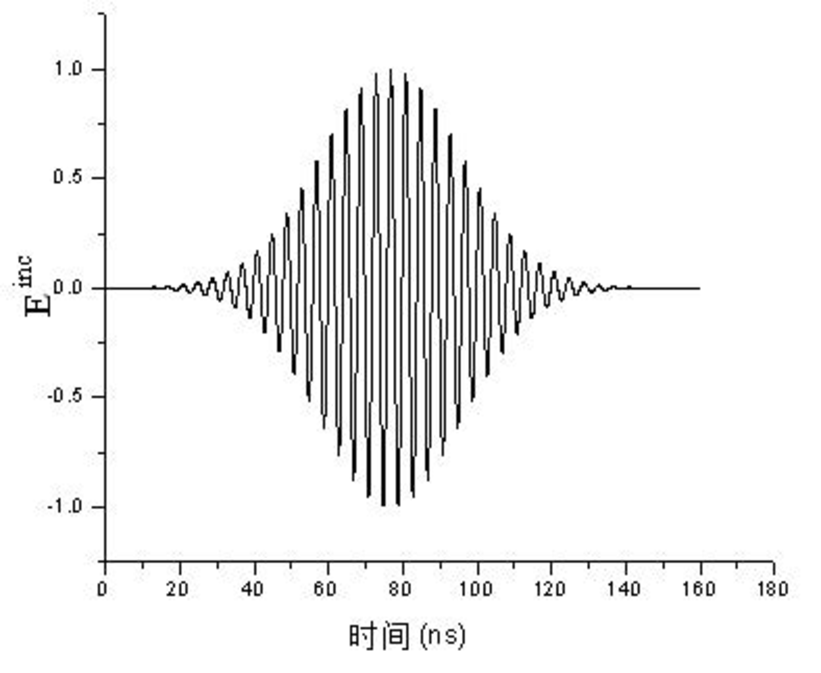
\includegraphics[width=7.3cm]{picb.pdf}
        \subcaption{aa1}
		\label{picb}
    \end{subfigure}
	\begin{subfigure}[b]{0.49\linewidth}
		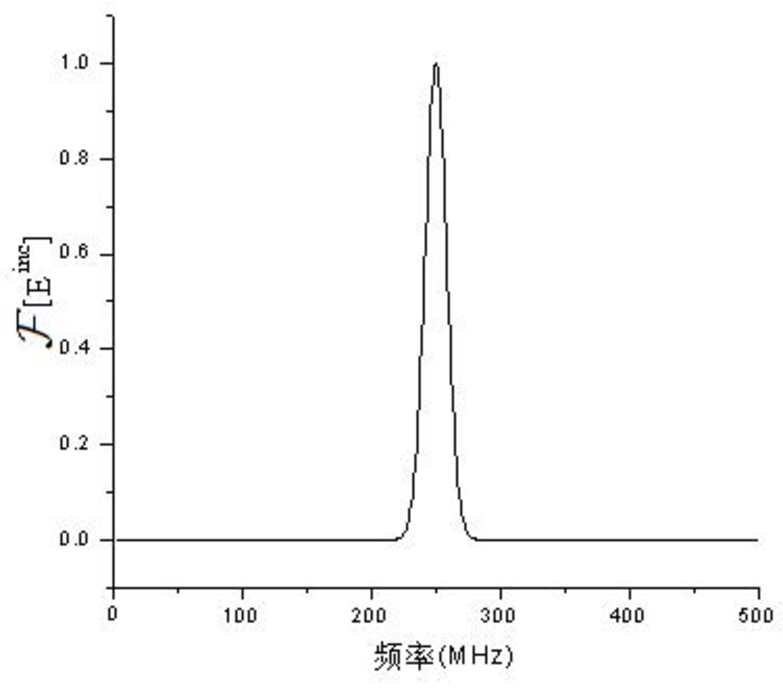
\includegraphics[width=6.41cm]{picc.pdf}
        \subcaption{aa2}
		\label{picc}
    \end{subfigure}
	\caption{电动汽车无序充电时各个时刻的充电功率。}
	\label{fig1}
\end{figure}

值得一提的是,当采用区间算法进行优化时,潮流计算所得的中间量(如节 电压、线路潮流),及最终得到的目标函数均为区间数。

\section{本章小结}
总结。
